\documentclass{beamer}
\usepackage{amsmath}%
\usepackage{amsfonts}%
\usepackage{amssymb}%
\usepackage{amsthm}%
\usepackage{graphicx}
\graphicspath{ {./Figures/} }
%\usepackage{hyperref}

\usepackage{graphicx}
\usepackage{subfig}

\usepackage[english]{babel}
\usepackage[utf8]{inputenc}

\usepackage{multicol}
%\usepackage{natbib}%
\usepackage{units}

\usepackage{stmaryrd}
\usepackage{gensymb}
\usepackage{bibentry}
\usepackage{accents}

%\usepackage{booktabs}

\usepackage{tensor}
\usepackage[bbgreekl]{mathbbol}
\usepackage{bm}
\usepackage{ulem}

% FANCY TABLES
\usepackage{booktabs}
\usepackage{multirow}
\usepackage{threeparttable}

%\usetheme{Luebeck}
\usetheme{Madrid}
%\usetheme{CambridgeUS}
%\usetheme{Pittsburgh}
%\usetheme{default}
%\mode<presentation>

%FOR CAMBRIDGE US THEME -- red bullets/captions in itemize environment
\setbeamercolor{item projected}{bg=black}
\setbeamertemplate{enumerate items}[default]
\setbeamertemplate{navigation symbols}{}
\setbeamercovered{transparent}

\setbeamercolor*{enumerate item}{fg=black}
\setbeamercolor*{enumerate subitem}{fg=black}
\setbeamercolor*{enumerate subsubitem}{fg=black}

\setbeamercolor{block title}{fg=black}
\setbeamercolor{caption name}{fg=black}

\title[Mechanika]{Inverzné Kyvadlo}
\author[Skupina Z] {Marek Mikloš, Ondřej Kureš, Ladislav Trnka \\ }
\institute[Charles University]{Charles University, Czech Republic}
\date{\today}

\begin{frame}
\titlepage
\bibliographystyle{plain}
\nobibliography{vit-prusa}
\end{frame}


\let\newblock\relax

\newcommand{\smallbibentry}[1]{{\tiny \bibentry{#1}}}

% \AtBeginSection[]
% {
%   \begin{frame}
% %    \frametitle{Outline}
%     \tableofcontents[currentsection]
%   \end{frame}
% }

\begin{document}



% \begin{frame}
%   \frametitle{Outline}
%   \tableofcontents
% \end{frame}

\section*{Úvod}
\label{sec: Int}


\begin{frame}
 
 \frametitle{Úvod}
 \begin{center}
 Cart and pole apparatus, tiltmeter, Kapitza's pendulum.\\    
 Newtonovský pohľad, Lagrangeov pohľad.\\
 Mathieuho rovnica.\\
 Perturbačná metóda určenia hraníc, $\alpha(\beta)$ \\
 \end{center}

 \begin{equation*}
\mathcal{L}=_{def}T-V=\frac{1}{2}m(l^2(\frac{d\theta}{dt})^2+(\frac{d\xi}{dt})^2+2l\sin\theta(\frac{d\xi}{dt})(\frac{d\theta}{dt}))-mg(\xi-lcos{\theta})
 \end{equation*}

 \begin{equation*}
 -\frac{d}{dt}(\frac{\partial\mathcal{L}}{\partial\dot{\bar{q_{i}}}})+ \frac{\partial\mathcal{L}}{\partial{}q_{i}}=0
 \end{equation*}
 
 \begin{equation*}
 \frac{\mathrm{d^2\theta} }{\mathrm{d} t^2}+(\frac{g}{l}-\frac{A{\Omega}^2}{l}cos{\Omega t})\theta=0
 \end{equation*}
 
\end{frame}
 

\section*{Záver}
\label{sec:Záver}

\begin{frame}
\frametitle{Záver}


\begin{figure}
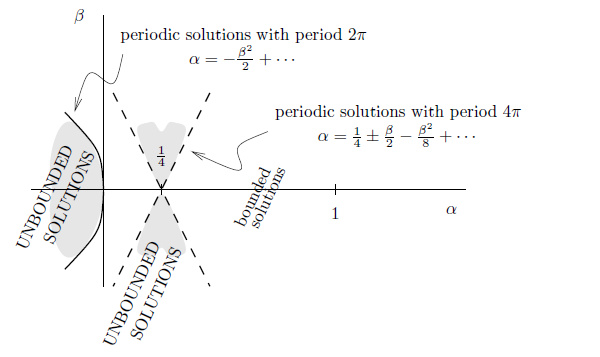
\includegraphics[scale=0.45]{Boundary-graph.png}
\end{figure}
Ak sú hodnoty parametrov $\alpha$ a $\beta$ z tmavej oblasti so stredom v bode $\alpha=\frac{1}{4}$, potom môže byť kyvadlo destabilizované osciláciou pivotu.
Pre vhodne zvolené hodnoty parametrov $\alpha$, $\beta$ dosiahneme stabilizáciu kyvadla v hornej časti, teda hodnoty týchto parametrov sa nachádzajú na grafe v bielej oblasti. Nutnou podmienkou stability je vhodne zvolená frekvencia kmitov pivotu:
 
\begin{equation*}
\frac{A}{l}\frac{\Omega}{\omega_0}\geq \sqrt{2}.
\end{equation*}  
 

\end{frame}




\end{document}

%
%
%
%
% DOCUMENT ENDS HERE
%
%
%
%